\documentclass[11pt]{article}
\usepackage[utf8]{inputenc}
\usepackage[T1]{fontenc}
\usepackage[margin=1in]{geometry}
\usepackage{amsmath,amssymb,amsthm}
\usepackage{graphicx}
\usepackage{booktabs}
\usepackage{tabularx}
\usepackage{listings}
\usepackage{upquote}
\usepackage{xcolor}
\usepackage{hyperref}
\hypersetup{colorlinks=true, linkcolor=blue, citecolor=blue, urlcolor=blue}

% generated by scripts/desi_dr2_bao/make_paper_inputs.py -- do not edit
\newcommand{\CambHrd}{-0.011}
\newcommand{\CambMassless}{$2.3\times10^{-11}$}
\newcommand{\CambMaxShift}{0.032}
\newcommand{\CambOm}{+0.032}
\newcommand{\CambRd}{147.1027}
\newcommand{\CambVersion}{2.0.4}
\newcommand{\CambW}{-0.008}
\newcommand{\CambWOm}{+0.032}
\newcommand{\CorrEmcee}{-0.9230}
\newcommand{\CorrFisher}{-0.9234}
\newcommand{\CorrGrid}{-0.9239}
\newcommand{\DOneHrd}{101.887}
\newcommand{\DOneHrdPull}{+0.067}
\newcommand{\DOneOm}{0.29498}
\newcommand{\DOneOmPull}{-0.0013}
\newcommand{\DOneOmSd}{0.01469}
\newcommand{\DOneWOm}{0.29305}
\newcommand{\DOneWOmPull}{+0.0033}
\newcommand{\DOneWhrd}{101.69}
\newcommand{\DOneWhrdPull}{-0.0021}
\newcommand{\DOneWw}{-0.9896}
\newcommand{\DOneWwPull}{+0.0025}
\newcommand{\DeltaHrd}{-0.36}
\newcommand{\DeltaOm}{+0.00283}
\newcommand{\EmGridMax}{0.0094}
\newcommand{\EmceeVersion}{3.1.6}
\newcommand{\EssMin}{14282}
\newcommand{\FitGenerated}{2026-09-27 19:14:42}
\newcommand{\FitSha}{4380af6d0e1ed743}
\newcommand{\GLdiff}{$2.4\times10^{-15}$}
\newcommand{\GridEdgeMax}{$2.7\times10^{-8}$}
\newcommand{\GridNthree}{141}
\newcommand{\GridNtwo}{601}
\newcommand{\LCDMchi}{10.271}
\newcommand{\LeanSha}{3b451bd5a93d682c}
\newcommand{\LeanStamp}{2026-09-27 17:59:28}
\newcommand{\LeanToolchain}{leanprover/lean4:v4.34.0-rc2}
\newcommand{\LedgerAudited}{6}
\newcommand{\LedgerBlock}{0}
\newcommand{\LedgerClaims}{25}
\newcommand{\LedgerFlag}{0}
\newcommand{\LedgerPreFlag}{6}
\newcommand{\LedgerPreRc}{1}
\newcommand{\LedgerRc}{0}
\newcommand{\LedgerTierA}{6}
\newcommand{\NCfiveAbove}{6}
\newcommand{\NCfiveAboveList}{202: 0.022, 208: 0.08, 210: 0.067, 212: 0.0088, 215: 0.0034, 218: 0.007}
\newcommand{\NCfiveMaxPte}{0.080}
\newcommand{\NCfiveN}{20}
\newcommand{\NCriteria}{14}
\newcommand{\NCriteriaTrue}{14}
\newcommand{\NstepsOverTauMin}{9.0}
\newcommand{\Orad}{$9.05\times10^{-5}$}
\newcommand{\PreregSha}{723cd27d3e5e198e}
\newcommand{\RadHrd}{+0.013}
\newcommand{\RadOm}{-0.046}
\newcommand{\RadW}{-0.0016}
\newcommand{\RadWOm}{-0.045}
\newcommand{\ShiftInd}{0.167}
\newcommand{\ShiftNestOwn}{0.237}
\newcommand{\ShiftNestPrereg}{0.231}
\newcommand{\SigIndOwn}{0.01700}
\newcommand{\SigNestOwn}{0.01194}
\newcommand{\SystMaxShift}{0.046}
\newcommand{\TauMax}{44.3}
\newcommand{\Verdict}{PASS}
\newcommand{\WCDMchi}{9.041}
\newcommand{\WhrdMean}{99.83}
\newcommand{\WhrdStd}{1.73}
\newcommand{\NData}{13}
\newcommand{\ResLOm}{0.29781}
\newcommand{\ResLOmSd}{0.00856}
\newcommand{\ResLHrd}{101.530}
\newcommand{\ResLHrdSd}{0.732}
\newcommand{\ResWOm}{0.29713}
\newcommand{\ResWOmSd}{0.00896}
\newcommand{\ResWw}{-0.9164}
\newcommand{\ResWwSd}{0.0787}
\newcommand{\MaxAbsPull}{0.037}
\newcommand{\MaxWidthDevPct}{0.9}

\makeatletter\def\rawinput#1{\@@input #1 }\makeatother

\newtheorem{theorem}{Theorem}

\lstdefinelanguage{Lean4}{
  morekeywords={theorem,def,noncomputable,import,namespace,end,open,by,fun},
  morecomment=[l]{--},
  morecomment=[s]{/-}{-/},
  sensitive=true,
}
\lstset{basicstyle=\small\ttfamily, language=Lean4, columns=fullflexible, breaklines=true,
  extendedchars=true, inputencoding=utf8, upquote=true,
  literate={ℝ}{{$\mathbb{R}$}}1 {≤}{{$\le$}}1 {⁻¹}{{$^{-1}$}}2 {∫}{{$\int$}}1}

\title{DESI DR2 BAO Alone: An Independent, Preregistered Reproduction of the\\
Flat-$\Lambda$CDM and Flat-$w$CDM Constraints, a DR1$\to$DR2 Consistency Check,\\
and a Kernel-Verified Model Skeleton}
\author{AutoevolveAI / ANSE Research Pipeline\\
\small Model-generated with Claude Code (automated pipeline)}
\date{September 27, 2026}

\begin{document}
\sloppy\emergencystretch=3em
\maketitle

\begin{abstract}
We re-derive the BAO-only cosmological constraints of the DESI DR2 release
\cite{desi2025dr2} from its public Gaussian BAO likelihood (\NData{} points,
full covariance). The targets, tolerances, estimator and every control were
written in a preregistration and frozen before any fit
(sha256 prefix \texttt{\PreregSha}). The primary estimator is the posterior
mean under DESI's flat priors, sampled with \texttt{emcee}~\EmceeVersion. We
obtain $\Omega_m=\ResLOm\pm\ResLOmSd$ and $hr_d=\ResLHrd\pm\ResLHrdSd$~Mpc in flat
$\Lambda$CDM, and $\Omega_m=\ResWOm\pm\ResWOmSd$, $w=\ResWw\pm\ResWwSd$ in flat
$w$CDM. The largest deviation from DESI's quoted values is \MaxAbsPull{}
published standard deviations, and every width agrees to within
\MaxWidthDevPct\%.

An independent grid posterior agrees with the MCMC to \EmGridMax{} MCMC
standard deviations. The minimum is $\chi^2_{\min}=\LCDMchi$ on 11 degrees
of freedom (DESI: 10.2), and the $\Omega_m$--$hr_d$ correlation is
$r=\CorrEmcee$ (DESI: $-0.92$). All five positive controls behave as
required, and all five negative controls fail as required. All
\NCriteria{} preregistered criteria pass.

Running DR1 through the same pipeline gives a shift
$\Delta\Omega_m=\DeltaOm$, which is $\ShiftNestPrereg\,\sigma$ under an
ideal-nesting error. A CAMB~\CambVersion{} cross-check and a radiation
variant bound the error from omitting radiation and neutrino mass in our
primary model: no parameter moves by more than \SystMaxShift\,$\sigma$.

Six Lean~4 theorems about the fitted $w$CDM background are kernel-checked
with exactly the trusted axioms: positivity of $E(z)$ over the full
$w$ prior, exact nesting with $\Lambda$CDM at $w=-1$, and strict
monotonicity of the comoving-distance integral. This is a reproduction, not
a new cosmological result.
\end{abstract}

\section{Introduction}

A measurement of the baryon acoustic oscillation (BAO) feature at
redshift~$z$ constrains two ratios: the transverse comoving distance
$D_M(z)/r_d$ and the Hubble distance $D_H(z)/r_d=c/(H(z)\,r_d)$, where
$r_d$ is the sound horizon at the drag epoch. DESI DR2 \cite{desi2025dr2}
reports these ratios in seven redshift bins. From them alone, it quotes the
following for flat $\Lambda$CDM (its eq.~17):
\[
\Omega_m=0.2975\pm0.0086,\qquad hr_d=(101.54\pm0.73)\ \mathrm{Mpc},\qquad r=-0.92,
\]
For flat $w$CDM (its Table~V, row ``DESI'') it quotes
$\Omega_m=0.2969\pm0.0089$ and $w=-0.916\pm0.078$.

An earlier exercise in this pipeline re-fit the DR1 release
\cite{desi2024vi}. That exercise compared a $\chi^2$ minimum with DESI's
posterior mean. At DR1 precision the difference is harmless, but it is the
wrong estimator. Here we match the estimator DESI states it uses. DR2
Sec.~V says: ``For 1D marginalized posterior results we quote the mean and
standard deviation when the distributions are symmetric.'' We also extend
the model to $w$CDM, and we measure the DR1$\to$DR2 shift with the same
code.

The whole exercise is preregistered, and the machine-readable record lives
in the accompanying repository:
\begin{itemize}
\item \texttt{results/desi\_dr2\_bao/preregistration.json}: the targets,
tolerances, estimator and every control;
\item \texttt{results/desi\_dr2\_bao/fit.json}: every number in this paper
(sha256 prefix \texttt{\FitSha});
\item \texttt{results/desi\_dr2\_bao/ledger/}: the tier-capped claim ledger.
\end{itemize}

\section{Data}

We use \texttt{desi\_gaussian\_bao\_ALL\_GCcomb\_\{mean,cov\}.txt} from the
DESI DR2 BAO release. The local data README attributes it to
\cite{desi2025dr2}. Its sha256 digests are fixed in the preregistration and
were checked again at fit time and when this paper's tables were generated.
Table~\ref{tab:data} is produced directly from these files.

The file means match Table~IV of \cite{desi2025dr2} (v3) to its rounding,
and $\sqrt{\mathrm{diag}\,C}$ matches the tabulated errors to within about
1.5\%. There is one caveat. The file's $D_M$--$D_H$ correlation coefficients
differ from Table~IV for some bins. For LRG3+ELG1 the file gives $-0.347$,
while Table~IV gives $-0.416$ in v3 and $-0.425$ in v1. We fit the file,
because it is the likelihood DESI distributes, and we record the difference
as a caveat.

For the DR1 comparison we use the DR1 files
\texttt{desi\_2024\_gaussian\_bao\_ALL\_GCcomb\_\{mean,cov\}.txt}
\cite{desi2024vi}, which have 12 points.

\begin{table}[h]
\centering
\caption{DESI DR2 Gaussian BAO likelihood as fitted. The error column is
$\sqrt{C_{ii}}$ from the covariance file. Correlations between $D_M$ and
$D_H$ in the same bin are included in the fit.}
\label{tab:data}
\begin{tabular}{cccc}
\toprule
$z_{\rm eff}$ & quantity & value & $\sqrt{C_{ii}}$ \\
\midrule
\rawinput{gen_data_table.tex}
\bottomrule
\end{tabular}
\end{table}

\section{Model and method}

The primary model, fixed in the preregistration, is flat, with matter and
dark energy only:
\begin{equation}
E^2(z)=\frac{H^2(z)}{H_0^2}=\Omega_m(1+z)^3+(1-\Omega_m)(1+z)^{3(1+w)},
\end{equation}
with $w=-1$ for $\Lambda$CDM. The distances are
\[
D_M=\frac{c}{100\ \mathrm{km\,s^{-1}\,Mpc^{-1}}}\int_0^z\frac{dz'}{E(z')},
\qquad
D_H=\frac{c}{100\,E(z)}\ \text{(same units)},
\]
and both are divided by $hr_d$ in Mpc. The isotropic distance is
$D_V=[z\,D_M^2D_H]^{1/3}$.

The priors are flat, following DESI \cite{desi2024vi} (Table~2):
$\Omega_m\sim U[0.01,0.99]$, $hr_d\sim U[10,1000]$~Mpc and
$w\sim U[-3,1]$. DR2 states that its priors ``match those given in Table~2
of [38]''. We identify [38] as \cite{desi2024vi} from context; we did not
read the bibliography entry.

We use three estimators:
\begin{enumerate}
\item \textbf{Primary estimator.} The \texttt{emcee}~\EmceeVersion{}
posterior mean and standard deviation, with 32 walkers and seed 20260927.
The distance integral uses 96-point Gauss--Legendre quadrature, which agrees
with \texttt{scipy.integrate.quad} to \GLdiff{} at the prior corners. The
preregistered convergence rule requires $n_{\rm steps}\ge50\,\tau_{\max}$
and at least $10^4$ effective samples.
\item \textbf{Grid posterior.} An independent grid posterior over the same
priors, with $\GridNtwo^2$ points for $\Lambda$CDM and $\GridNthree^3$
points for $w$CDM, spanning $\pm10$ Fisher standard deviations. The largest
marginal mass in any edge cell is \GridEdgeMax.
\item \textbf{$\chi^2$ minimum.} A Nelder--Mead $\chi^2$ minimum with the
Fisher matrix evaluated there. It is used only against DESI's best-fit
$\chi^2$ and in the controls.
\end{enumerate}

All six MCMC runs converged at 20{,}000 steps. The runs are DR2 and DR1, each
in $\Lambda$CDM and $w$CDM, plus the two DR2 radiation variants. The largest
autocorrelation time is $\tau_{\max}=\TauMax$ and the smallest effective
sample size is \EssMin. Two identical 300-step runs reproduced bit for bit.

\section{Preregistration}

The preregistration was written before any fit of this problem (revision r2,
2026-09-27 15:55~UTC). It is frozen: no file of it was modified afterwards,
and its sha256 is re-checked by every analysis script. It fixes the
following:
\begin{itemize}
\item the four scored targets;
\item two secondary targets: DESI's best-fit $\chi^2/\mathrm{dof}=10.2/11$
\cite{desi2025dr2} (Sec.~III.C.1) and the $\Omega_m$--$hr_d$ correlation
$r=-0.92$;
\item the pass rule;
\item every control in Table~\ref{tab:controls}.
\end{itemize}

The pass rule is:
\begin{itemize}
\item every target within $0.5$ published standard deviations of the
published value;
\item every width ratio $\sigma_{\rm ours}/\sigma_{\rm pub}$ in $[0.8,1.2]$;
\item $|r+0.92|\le0.05$;
\item $|\chi^2_{\min}-10.2|\le0.5$;
\item all controls behaving as specified;
\item every MCMC run converged;
\item all data sha256 digests matching.
\end{itemize}

The DR2 $w$CDM value of $hr_d$ is report-only. No BAO-only DR2 value was
found in \cite{desi2025dr2} or in \cite{lodha2025}, so it has no target.

\section{Controls}

Following this pipeline's rule that every experiment runs positive and
negative controls before its numbers count, the preregistration makes the
controls binding: if any positive control fails or any negative control
passes, no target agreement may be reported as a success. The script
\texttt{assemble\_fit.py} applies this rule mechanically. The outcomes are listed in
Table~\ref{tab:controls}. The noisy mocks in PC3 are 500 draws from
$\mathcal N(\mathrm{model}(0.2975,101.54),C_{\rm DR2})$. Their pulls use the
Fisher standard deviation at the truth point.

NC5 passes its preregistered criterion only in aggregate. \NCfiveAbove{} of
the \NCfiveN{} individual scrambled-covariance fits have PTE $>10^{-3}$
(as seed: PTE, these are \NCfiveAboveList; the largest is \NCfiveMaxPte). A scrambled
covariance is therefore often still an acceptable fit on its own. This
control tests the covariance ordering in aggregate and has limited power for
any single realisation.

\begin{table}[h]
\centering\small
\caption{Preregistered controls. The threshold column gives the
preregistered criterion for each control. ``As required'' means pass for a
positive control and fail for a negative one. All values are copied from
\texttt{controls.json}.}
\label{tab:controls}
\begin{tabularx}{\textwidth}{>{\raggedright}p{3.4cm}>{\raggedright}X>{\raggedright}X l}
\toprule
control & threshold & measured & outcome \\
\midrule
\rawinput{gen_controls_table.tex}
\bottomrule
\end{tabularx}
\end{table}

\section{Results}

\begin{table}[h]
\centering\small
\caption{DR2 BAO-only results against the preregistered targets. The
``pull'' column is (ours $-$ published)/$\sigma_{\rm pub}$. The ``width''
column is $\sigma_{\rm ours}/\sigma_{\rm pub}$. Values are generated from
\texttt{fit.json} (generated \FitGenerated~UTC).}
\label{tab:results}
\begin{tabular}{lccccc}
\toprule
parameter & emcee mean$\pm$sd & grid mean$\pm$sd & DESI DR2 \cite{desi2025dr2} & pull & width \\
\midrule
\rawinput{gen_results_table.tex}
\bottomrule
\end{tabular}
\end{table}

Table~\ref{tab:results} shows the four scored targets, and the verdict under
the preregistered rule is \textbf{\Verdict}: \NCriteriaTrue{} of
\NCriteria{} criteria hold. The remaining quantities are:
\begin{itemize}
\item \textbf{$\Lambda$CDM secondary targets.} The minimum is
$\chi^2_{\min}=\LCDMchi$ on 11~dof. The $\Omega_m$--$hr_d$ correlation is
$r=\CorrEmcee$ from emcee, \CorrGrid{} from the grid and \CorrFisher{} from
the Fisher matrix.
\item \textbf{$w$CDM.} The minimum is $\chi^2_{\min}=\WCDMchi$ on 10~dof.
The report-only value is $hr_d=\WhrdMean\pm\WhrdStd$~Mpc.
\end{itemize}
Figure~\ref{fig:post} shows the posteriors.

\begin{figure}[h]
\centering
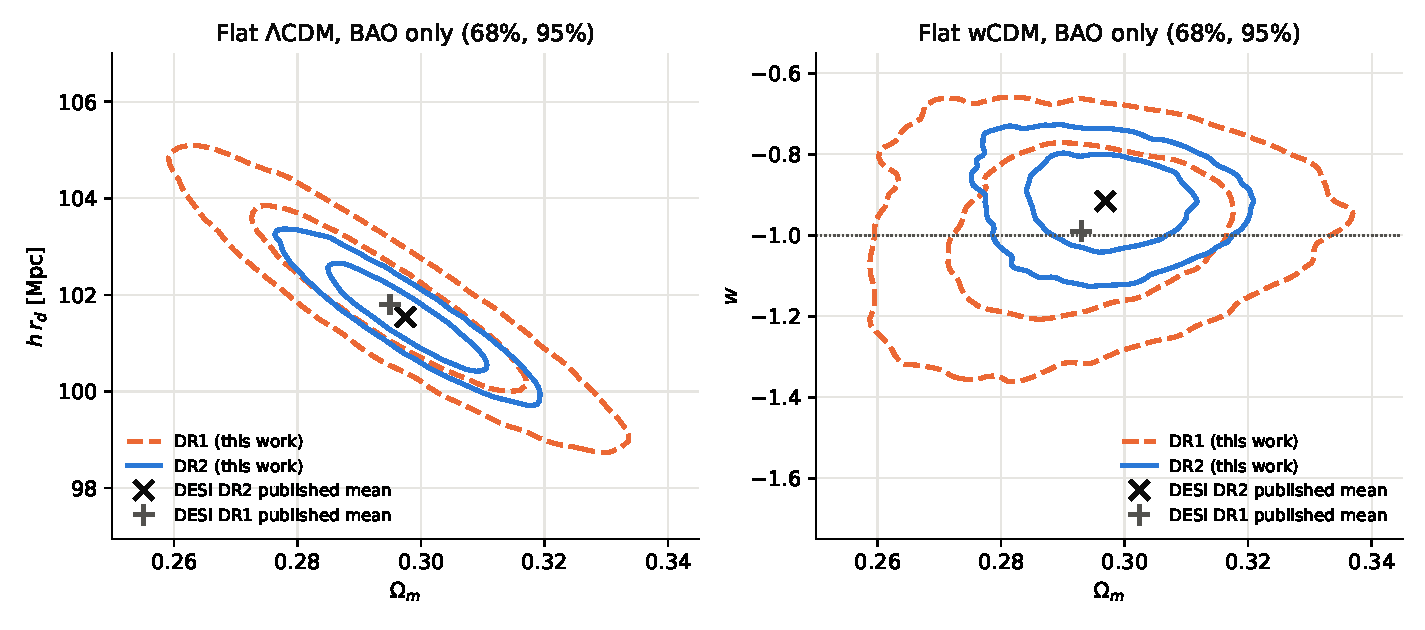
\includegraphics[width=0.9\textwidth]{../../results/desi_dr2_bao/desi_dr2_bao_posteriors.pdf}
\caption{68\% and 95\% posterior contours from emcee. Left: flat
$\Lambda$CDM in ($\Omega_m$, $hr_d$). Right: flat $w$CDM in ($\Omega_m$,
$w$). Each panel shows DR2 and DR1 (this work) and marks DESI's published
means. Figure produced by \texttt{scripts/desi\_dr2\_bao/make\_figure.py} from
the chains in \texttt{results/desi\_dr2\_bao/chains/}.}
\label{fig:post}
\end{figure}

\paragraph{DR1 instrument check.} The same pipeline, run on DR1, gives the
following, with the pull relative to \cite{desi2024vi} eq.~(4.1) or (5.1)
in parentheses:
\begin{itemize}
\item $\Lambda$CDM: $\Omega_m=\DOneOm$ (pull \DOneOmPull) and
$hr_d=\DOneHrd$~Mpc (pull \DOneHrdPull);
\item $w$CDM: $\Omega_m=\DOneWOm$ (pull \DOneWOmPull) and $w=\DOneWw$
(pull \DOneWwPull).
\end{itemize}
The DR1 $w$CDM value $hr_d=\DOneWhrd$~Mpc (pull \DOneWhrdPull) is compared
against the value in \cite{desi2024vi}, Sec.~6 (printed p.~36):
$r_dh=(101.7^{+2.9}_{-3.5})$~Mpc ($w$CDM). This page was re-fetched in the
fix round and matches the literature-review transcription.

\paragraph{DR1$\to$DR2 consistency.} From our two posteriors we find
$\Delta\Omega_m=\DeltaOm$ and $\Delta(hr_d)=\DeltaHrd$~Mpc. The published
difference, derived from the two papers, is $0.2975-0.295=+0.0025$; DESI
does not quote it. DR1 is a subset of DR2, so the primary error is the
ideal-nesting approximation
$\sigma_{\rm nest}=\sqrt{\sigma_{\rm DR1}^2-\sigma_{\rm DR2}^2}$. With the
preregistered $\sigma_{\rm nest}=0.01229$ the shift is
$\ShiftNestPrereg\,\sigma$. With our own $\sigma_{\rm nest}=\SigNestOwn$ it
is $\ShiftNestOwn\,\sigma$. Treating the releases as independent
($\sigma=\SigIndOwn$) gives $\ShiftInd\,\sigma$. All three preregistered
shift predictions pass.

\paragraph{Modelling systematics.} We ran two checks.
\begin{itemize}
\item \textbf{CAMB with massless neutrinos.} CAMB~\CambVersion{}, run with
massless neutrinos and its own $\Omega_r$, reproduces our quadrature $D_M$
and $H$ to \CambMassless{} relative, for $w=-1$ and $w=-0.9$.
\item \textbf{CAMB with a 0.06~eV neutrino.} We fitted our primary model,
which has no radiation and no neutrino mass, to a noiseless CAMB data vector
with one 0.06~eV neutrino. The fitted $\Omega_m$ shifts by \CambOm\,$\sigma$
and $hr_d$ by \CambHrd\,$\sigma$ in $\Lambda$CDM. In $w$CDM, $w$ shifts by
\CambW\,$\sigma$.
\end{itemize}
The preregistered radiation variant ($\Omega_r=$~\Orad) shifts $\Omega_m$ by
\RadOm\,$\sigma$, $hr_d$ by \RadHrd\,$\sigma$ and $w$ by \RadW\,$\sigma$.
Every shift is far below the $0.3\,\sigma$ flag. CAMB also gives the
Planck-2018 best-fit sound horizon $r_{\rm drag}=\CambRd$~Mpc, matching the
orchestrator's independent positive control.

\section{Lean 4 formalization}\label{sec:lean}

The file \texttt{formal/ANSE/DESI\_DR2\_wCDM.lean} (sha256 prefix
\texttt{\LeanSha}, toolchain \texttt{\LeanToolchain}) formalizes the
background model that the fit evaluates. It takes
\texttt{dr2\_model.e\_of\_z} with $\Omega_r=0$ and the comoving distance
$\int_0^z dt/E(t)$. The exponent $3(1+w)$ is a real power
(\texttt{Real.rpow}), as in \texttt{numpy}. Imports are pinned to the
locally built Mathlib subset plus \texttt{ANSE.BAO\_FlatLCDM} from the DR1
exercise. The definitions and theorem statements below are extracted
verbatim from the file; proofs are elided.

\begin{lstlisting}
noncomputable def E2 (Om w z : ℝ) : ℝ :=
  Om * (1 + z) ^ 3 + (1 - Om) * (1 + z) ^ (3 * (1 + w))

noncomputable def E (Om w z : ℝ) : ℝ := Real.sqrt (E2 Om w z)

noncomputable def Dc (Om w z : ℝ) : ℝ := ∫ t in (0:ℝ)..z, (E Om w t)⁻¹

theorem E2_pos {Om w z : ℝ} (hOm0 : 0 < Om) (hOm1 : Om < 1) (hz : 0 ≤ z) :
    0 < E2 Om w z := ...

theorem E_pos {Om w z : ℝ} (hOm0 : 0 < Om) (hOm1 : Om < 1) (hz : 0 ≤ z) :
    0 < E Om w z := ...

theorem E_w_neg_one (Om z : ℝ) : E Om (-1) z = ANSE.BAOFlatLCDM.E Om z := ...

theorem E_strictMonoOn_of_neg_one_le {Om w : ℝ} (hOm0 : 0 < Om) (hOm1 : Om < 1)
    (hw : -1 ≤ w) : StrictMonoOn (E Om w) (Set.Ici (0 : ℝ)) := ...

theorem invE_continuousOn {Om w : ℝ} (hOm0 : 0 < Om) (hOm1 : Om < 1) :
    ContinuousOn (fun t => (E Om w t)⁻¹) (Set.Ici (0 : ℝ)) := ...

theorem Dc_strictMonoOn {Om w : ℝ} (hOm0 : 0 < Om) (hOm1 : Om < 1) :
    StrictMonoOn (Dc Om w) (Set.Ici (0 : ℝ)) := ...
\end{lstlisting}


The statements say the following:
\begin{itemize}
\item $E^2>0$ and $E>0$ for $0<\Omega_m<1$, $z\ge0$ and every real $w$, so
the whole prior box is covered, the phantom side included. This is a
\emph{preregistration deviation}: the lean\_plan stated the domain
$z>-1$. The delivered $z\ge0$ is strictly narrower. It still covers every
data redshift and the whole prior box. The file was left unchanged in the
fix round, so that the statement audit applies to the exact file that was
audited.
\item At $w=-1$ the $w$CDM $E$ equals the flat-$\Lambda$CDM $E$ of the DR1
formalization, so the two fits are exactly nested.
\item $E$ is strictly increasing on $[0,\infty)$ when $w\ge-1$. No claim is
made for $w<-1$, where the dark-energy term decreases.
\item $1/E$ is continuous on $[0,\infty)$.
\item $D_C$ is strictly increasing on $[0,\infty)$ for every real $w$. This
is an interval-integral result, not merely algebra.
\end{itemize}

The file carries its own \texttt{\#print axioms} lines. Compiling it with
\texttt{lake env lean} (return code 0, no errors or warnings, gate run
\LeanStamp~UTC) prints exactly:

\begin{lstlisting}[language={}]
'ANSE.DESIDR2wCDM.E2_pos' depends on axioms: [propext, Classical.choice, Quot.sound]
'ANSE.DESIDR2wCDM.E_pos' depends on axioms: [propext, Classical.choice, Quot.sound]
'ANSE.DESIDR2wCDM.E_w_neg_one' depends on axioms: [propext, Classical.choice, Quot.sound]
'ANSE.DESIDR2wCDM.E_strictMonoOn_of_neg_one_le' depends on axioms: [propext, Classical.choice, Quot.sound]
'ANSE.DESIDR2wCDM.invE_continuousOn' depends on axioms: [propext, Classical.choice, Quot.sound]
'ANSE.DESIDR2wCDM.Dc_strictMonoOn' depends on axioms: [propext, Classical.choice, Quot.sound]
\end{lstlisting}


\noindent There is no \texttt{sorryAx} and no axiom outside
$\{\texttt{propext},\texttt{Classical.choice},\texttt{Quot.sound}\}$. The
Elenchus scanner \texttt{elenchus\_check.py} reports ``no findings''. To
check that the scanner can detect a problem in this file, we built a copy in
which the proof of \texttt{E\_w\_neg\_one} is replaced by \texttt{sorry}.
Elenchus flags that copy \texttt{INHERITED\_SORRY} and exits with return
code~1 (\texttt{results/desi\_dr2\_bao/lean\_gate\_negative\_control.json}).

\paragraph{Claim ledger.} The ledger registers \LedgerClaims{} claims in
Elenchus's tier-capped format. Six are Tier~A (the theorems above) and
eight are Tier~B (our computations). Ten are Tier~L: five published
values and priors, and five comparisons against them, which rest on
citations. One is a Tier~C argument that the Lean definitions are faithful
to the code.

Before the statement audit, the gate reported 0 blocking findings and
\LedgerPreFlag{} flags, all \texttt{LEDGER\_UNAUDITED\_TIER\_A}, with
return code \LedgerPreRc. A workflow referee then audited the six Lean
statements against \texttt{dr2\_model.py}. That referee is an automated
model, not a person. It judged all six faithful
(\texttt{results/desi\_dr2\_bao/referee\_report.json}). Its verdicts are
recorded as audit objects on \LedgerAudited{} of the \LedgerTierA{} Tier~A
rows. Each object names the auditor as a model, and each is bound to the
sha256 of the audited Lean file.

With these audits the gate reports \LedgerBlock{} blocking findings and
\LedgerFlag{} flags, and its return code is \LedgerRc. Elenchus's flag text
asks for a \emph{person}'s certification, so this return code means
``model-referee audited''. A human statement audit is still outstanding.
Three mutations of the ledger were each caught as a block: a tier
inversion, a tampered evidence blob, and a kind over-claim.

\section{Limitations}

\begin{itemize}
\item \textbf{A reproduction, not a new constraint.} We use DESI's
likelihood, priors and estimator. Agreement is expected by construction. The
value of the exercise lies in the independent code path, the preregistration
and the controls.
\item \textbf{Different sampler and theory code.} We use \texttt{emcee} and
analytic quadrature, while DESI uses Cobaya Metropolis--Hastings with CAMB.
The physics missing from our primary model (radiation and a 0.06~eV
neutrino) moves no parameter by more than \SystMaxShift\,$\sigma$ (CAMB
check and radiation variant together).
\item \textbf{Covariance-file correlations.} The file's $D_M$--$D_H$
correlations differ from Table~IV of \cite{desi2025dr2} for LRG3+ELG1 and
ELG2. We fit the file.
\item \textbf{Prior source.} The source of the priors is inferred: we
identified ``[38]'' in \cite{desi2025dr2} from context.
\item \textbf{Table~V version.} The $w$CDM row of Table~V was read in v3
only. The $\Lambda$CDM targets are identical in v1 and v3.
\item \textbf{Nesting approximation.} $\sigma_{\rm nest}$ is an
ideal-nesting approximation. DESI's own DR1/DR2 correlation model is
$C=\sqrt{N_{\rm DR1}/N_{\rm DR2}}$ per tracer (0.61 for Ly$\alpha$), which
we did not reproduce.
\item \textbf{$w$CDM $hr_d$.} It is report-only, with no published target.
\item \textbf{Lean scope and audit.}
  \begin{itemize}
  \item The Lean theorems are facts about the model, not about the data or
  the fit.
  \item The Tier~A rows were audited for statement faithfulness by an
  automated model referee only, not by a person.
  \item $E^2>0$ and $E>0$ are proved for $z\ge0$, not for the preregistered
  $z>-1$ (a preregistration deviation, see Sec.~\ref{sec:lean}).
  \item The radiation variant is not formalized.
  \item The gate that ran is \texttt{scripts/desi\_dr2\_bao/lean\_gate.py}.
  It performs the same compile, \texttt{\#print axioms}, \texttt{sorryAx}
  and whitelist checks. The preregistration names
  \texttt{anse/formal/lean\_runner.py}, which was not used because it needs
  a \texttt{lake build} of the module.
  \end{itemize}
\item \textbf{Script edit after the runs (closed).} After the first chains
were written, \texttt{mcmc\_fit.py} received an annotation-only edit (a
return type). In the fix round all six chains and both grids were
regenerated from the current \texttt{mcmc\_fit.py} and
\texttt{grid\_posterior.py}. Every chain is bit-identical to its
predecessor (\texttt{np.array\_equal}), and both summaries are identical
apart from timestamps (\texttt{results/desi\_dr2\_bao/fixround\_rerun\_check.json}).
\end{itemize}

\section*{Acknowledgments}
This work uses public BAO likelihood products of the Dark Energy
Spectroscopic Instrument (DESI) collaboration. The analysis code, the Lean
formalization and this document were produced in the AutoevolveAI/ANSE
pipeline, orchestrated by Claude Code. Software:
emcee~\EmceeVersion, CAMB~\CambVersion, NumPy, SciPy, Astropy and Lean~4
with Mathlib.

\begin{thebibliography}{9}

\bibitem{desi2025dr2}
DESI Collaboration, ``DESI DR2 Results II: Measurements of Baryon Acoustic
Oscillations and Cosmological Constraints,'' arXiv:2503.14738 (v3, 9 Oct
2025; v1 checked for eq.~17 and Table~IV).

\bibitem{desi2024vi}
DESI Collaboration, ``DESI 2024 VI: Cosmological Constraints from the
Measurements of Baryon Acoustic Oscillations,'' arXiv:2404.03002 (v3).

\bibitem{lodha2025}
K.~Lodha et al., DESI DR2 extended dark-energy analysis, arXiv:2503.14743
(v2); title not transcribed in our literature review. Consulted only to
confirm that no BAO-only DR2 $w$CDM $hr_d$ value is given in the pages
returned.

\end{thebibliography}

\end{document}
